\documentclass[hidelinks,12pt,dvipsnames,border=2pt]{standalone}
%\usepackage[top=0.7in, bottom=0.8in, left=1in, right=1in]{geometry}
\usepackage{tikz}
\usepackage{hyperref}
\usetikzlibrary{arrows}
\usetikzlibrary{shapes}
\usepackage{enumitem}
\usepackage{bm}
\usepackage{mathdots}
\usepackage{amsmath}
\usepackage{tcolorbox}
\usetikzlibrary{shadings}
\usetikzlibrary{decorations.pathreplacing}
\usepackage{helvet}
\usepackage{url}
\usepackage{graphicx}
\usetikzlibrary{arrows.meta,positioning,fit,calc}
\renewcommand{\familydefault}{\sfdefault}


\usetikzlibrary{arrows,decorations.pathmorphing,backgrounds,fit,positioning,shapes.symbols,chains}

\begin{document}
	
% trim=left botm right top
\begin{tikzpicture}
\node at (0,0) {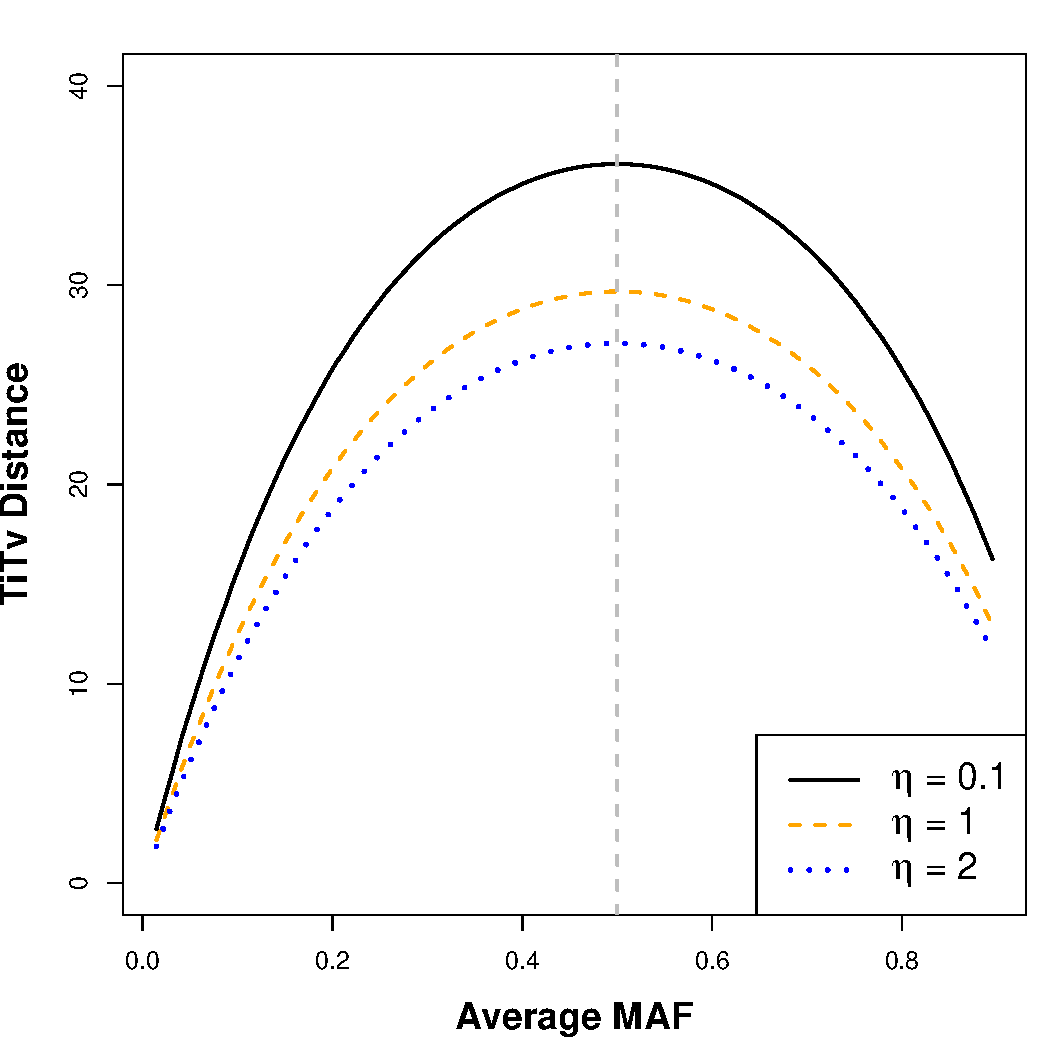
\includegraphics[clip,trim=0cm 0.2cm 0.4cm 0.91cm,width=\textwidth]{predicted_TiTv_distance-vs-Average_maf_new.pdf}};

\node[fill=white] at (5.1,-3.15) {\Large $\eta$};
\node[fill=white] at (5.1,-3.735) {\Large $\eta$};
\node[fill=white] at (5.1,-4.34) {\Large $\eta$};

\node[fill=white,draw=black!25,rounded corners=5,line width=0.3mm] at (1.39,0) {
	\begin{tabular}{c}
		\textbf{Maximum Distance} \\
		$\bar{f}_a = 0.5$
	\end{tabular}
};

\draw[-latex,line width=0.7mm] (1.39,5.115) -- (1.39,3.4);
\draw[-latex,line width=0.7mm,draw=orange!70] (1.39,4.3) -- (1.39,3.4);

\draw[-latex,line width=0.7mm,draw=orange!70] (1.39,3.4) -- (1.39,2.7); 
\draw[-latex,line width=0.7mm,draw=blue] (1.39,3.15) -- (1.39,2.7);

\end{tikzpicture}

\end{document}